\section{Results}

\subsection{Evaluation of clustering methods}

The goal of this evaluation is to find an accurat clustering method for working with news articles. The most suitable algorithm will then be used for the online approach of detecting changes in a news stream based on stories.


To begin the evaluation, we first compare six different clustering methods with each other. K-means is included as a baseline, to put the scores in relation to one of the most commonly used clustering algorithms. As we can see in figure \ref{fig:different_clusterings}, HDBSCAN provides together with K-means the highest accuracy compared to the others. One of the reason of the general low scores is the high-dimensionality of the test data.  

% TODO Explain why HDBSCAN is better than the rest

% TODO show plot with accuracy,  processing times and difference in clusters

Based on the results so far HDBSCAN appears to be the best candidate for our use case. The following parts of the evaluation will focus on HDBSCAN to get more insight into its performance and other properties.


The plots previously shown in the evaluation process were based on a sample size of 30 stories which amounts to roughly 1000 news articles. The low number of samples was due to the long processing times of some of the algorithms. Increasing the sample size results for both HDBSCAN and K-means in a small loss regarding the accuracy as can be seen in Figure \ref{fig:accuracy_kmeans_hdbscan}.

% Explain the loss in accuracy

\begin{figure}[h]
    \centering
    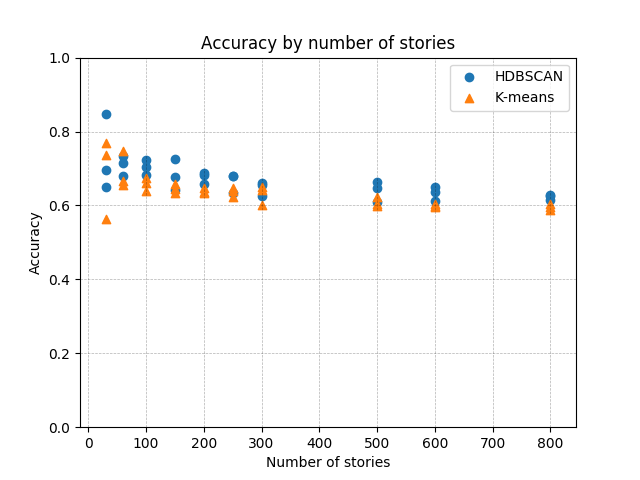
\includegraphics[width=0.5\textwidth]{accuracy_kmeans_hdbscan}
    \caption{Comparison of the average accuracy between K-means and HDBSCAN}
    \label{fig:accuracy_kmeans_hdbscan}
\end{figure}

\begin{figure}[h]
    \centering
    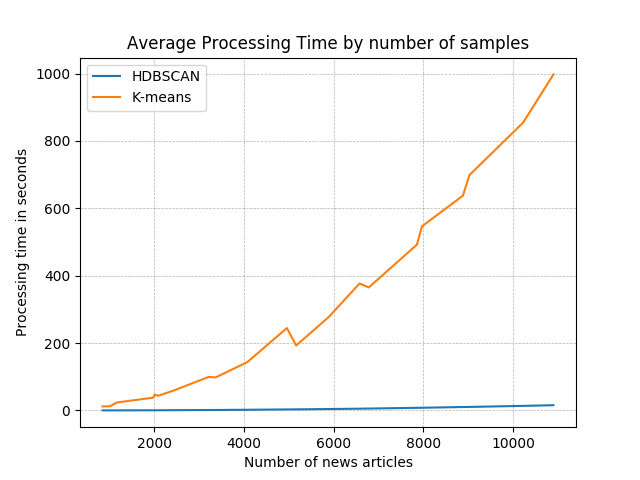
\includegraphics[width=0.5\textwidth]{processing_time_kmeans_hdbscan}
    \caption{Processing time in seconds }
    \label{fig:processing_time_kmeans_hdbscan}
\end{figure}

Being able to handle noise is one of the advantages of HDBSCAN has over the other previously tested clustering algorithms. It is reasonable to expect to have a lot of noise in the incoming stream of news articles, once the algorithm is applied in an online setting. However this evaluation is done with a labeled static dataset, containing a minimum amount of noise. The noise ratio shown in Figure \ref{fig:noise_ratio_samples} is much higher than we would expect from the test data. 

\begin{figure}[h]
    \centering
    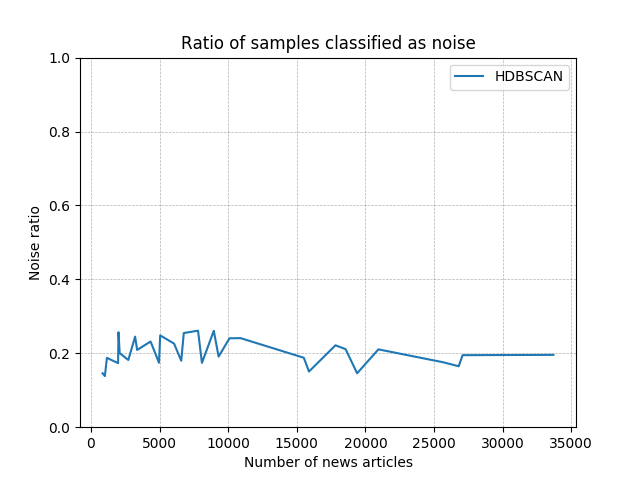
\includegraphics[width=0.5\textwidth]{noise_ratio_samples}
    \caption{Number of news articles classified as noise.}
    \label{fig:noise_ratio_samples}
\end{figure}

% Explain the high noise rate


\begin{figure}[h]
    \centering
    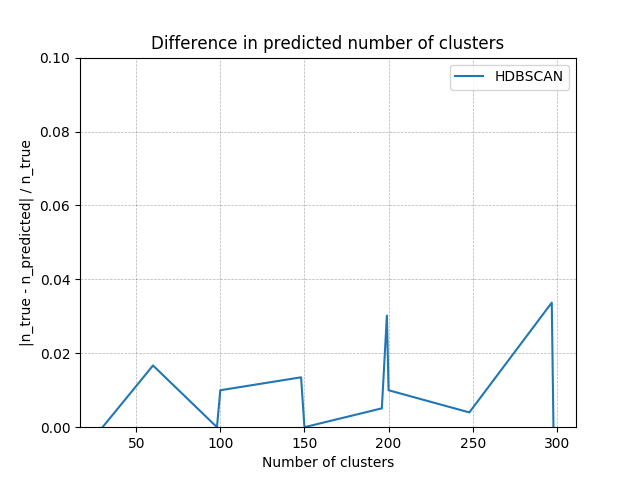
\includegraphics[width=0.5\textwidth]{cluster_difference_samples}
    \caption{Example of a parametric plot ($\sin (x), \cos(x), x$)}
    \label{fig:cluster_difference_samples}
\end{figure}